% section5_sensitivity.tex — Module C: Zhe
\section{Sensitivity to Prior Specification}\label{sec:sensitivity}

To assess whether posterior inference is driven by the data or the
prior, we compared three prior specifications for the standardised
regression coefficients $\beta_j$:

\begin{itemize}
    \item \textbf{Prior A} (baseline): $\beta_j \sim \mathcal{N}(0,\,10^2)$,
          $\sigma \sim \text{HalfNormal}(5)$ --- weakly informative.
    \item \textbf{Prior B} (diffuse): $\beta_j \sim \mathcal{N}(0,\,100^2)$,
          $\sigma \sim \text{HalfNormal}(50)$ --- ten times more diffuse.
    \item \textbf{Prior C} (stress test): $\beta_j \sim \mathcal{N}(0,\,0.01^2)$,
          $\sigma \sim \text{HalfNormal}(0.01)$ --- strongly informative near zero.
\end{itemize}

\subsection{Comparison of Priors A and B}

Table~\ref{tab:sensitivity} reports posterior means and 95\% credible
intervals under Priors A and B. The posterior means are virtually
identical across all three coefficients: the largest shift is
$|\Delta\bar{\beta}| = 0.0007$ for $\beta_0$, representing a change of
less than 0.1\% relative to the posterior standard deviation.
Credible interval widths change by at most 0.005 standard deviation
units. The overlaid posterior density plots (Figure~\ref{fig:sensitivity})
show near-perfect overlap between the two prior specifications.

\begin{table}[htbp]
    \centering
    \caption{Posterior means and 95\% credible intervals under Priors A and B.}
    \label{tab:sensitivity}
    \begin{tabular}{lrrrrl}
        \hline
        Parameter & A mean & A 95\% CrI & B mean & B 95\% CrI & $\Delta$mean \\
        \hline
        $\beta_0$ & $-0.001$ & $[-0.08,\; 0.08]$ & $0.000$  & $[-0.07,\; 0.08]$ & $+0.001$ \\
        $\beta_1$ & $0.639$  & $[0.56,\; 0.72]$  & $0.639$  & $[0.56,\; 0.72]$  & $<0.001$ \\
        $\beta_2$ & $-0.178$ & $[-0.26,\; -0.10]$& $-0.178$ & $[-0.26,\; -0.10]$& $<0.001$ \\
        \hline
    \end{tabular}
\end{table}

This stability demonstrates that the posterior is \emph{data-dominated}:
with 360 observations, the likelihood overwhelms both the weakly and the
very diffuse prior, and the data alone determine the posterior location
and spread.

\begin{figure}[htbp]
    \centering
    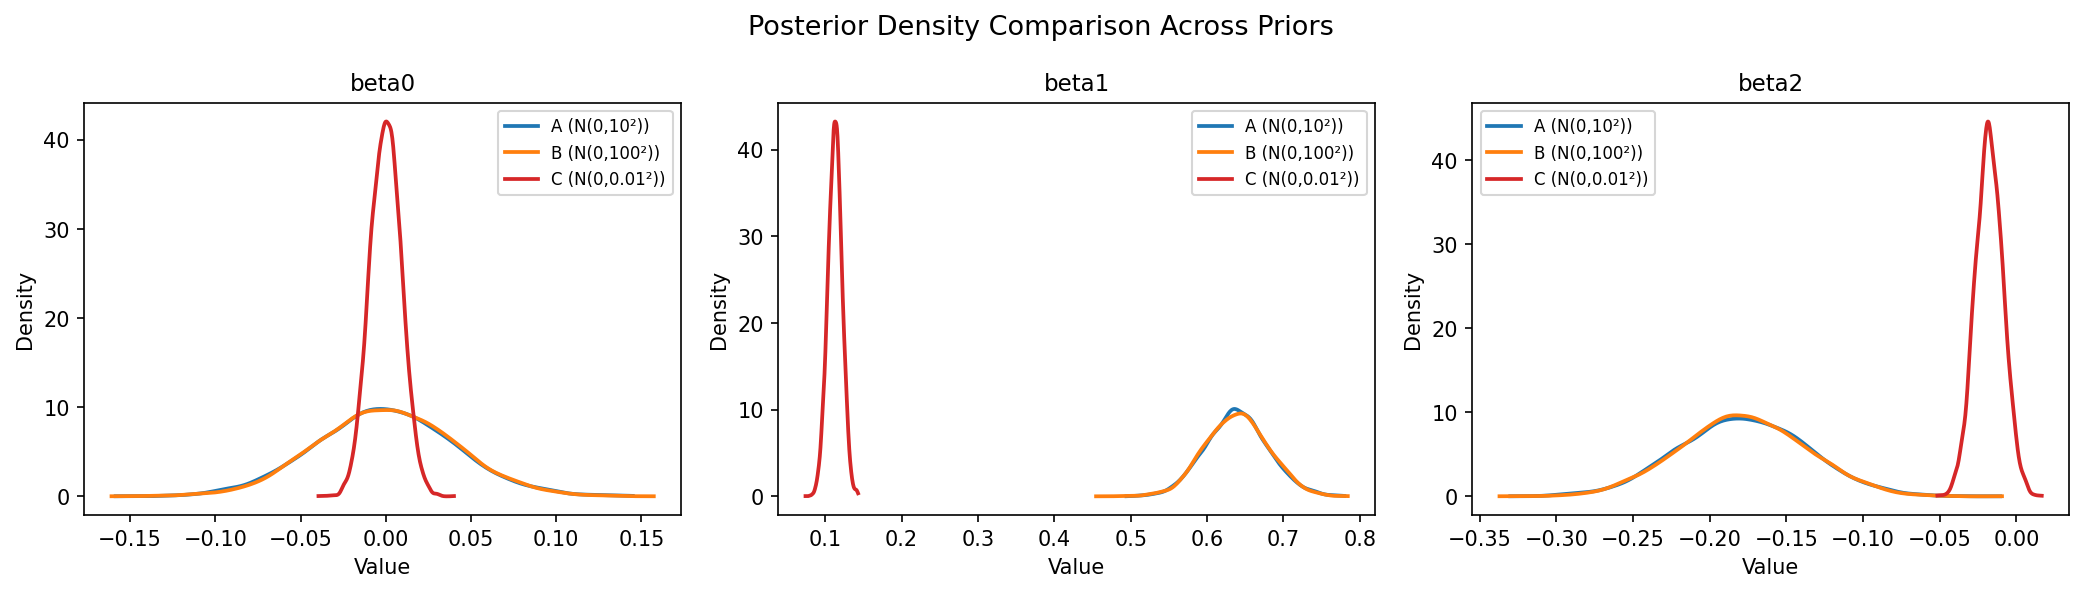
\includegraphics[width=\textwidth]{../results/figures/sensitivity_comparison.png}
    \caption{Overlaid posterior densities for $\beta_0$, $\beta_1$, $\beta_2$
    under Priors A (blue), B (orange), and C (red). Priors A and B yield
    near-identical posteriors; Prior C collapses all estimates toward zero.}
    \label{fig:sensitivity}
\end{figure}

\subsection{Stress Test: Prior C}

Under the strongly informative Prior C
($\beta_j \sim \mathcal{N}(0,\,0.01^2)$), the posteriors are pulled
sharply toward zero: $\hat{\beta}_1$ falls from $0.639$ to $0.113$ and
$\hat{\beta}_2$ from $-0.178$ to $-0.018$, with 95\% CrI widths
shrinking from $\approx 0.16$ to $\approx 0.04$ standard deviation
units. This confirms that a sufficiently informative prior \emph{can}
dominate the posterior regardless of the data.

\subsection{Conclusion}

The near-identical posteriors under Priors A and B, combined with the
marked contraction under Prior C, provide strong evidence that the
baseline analysis is \emph{data-dominated}. The 360-observation
likelihood is sufficiently informative to render the posterior robust
to reasonable variation in prior specification, and the conclusions
regarding the positive effect of temperature ($\hat{\beta}_1 = 0.639$)
and the negative effect of humidity ($\hat{\beta}_2 = -0.178$) on
daily bike-sharing demand are not an artefact of the prior choice.
